\section{Experiments}
\label{sec:experiments}

\paragraph{Setup.}
We use four benchmarks of RSIAT~\cite{rsiat}, each with seeds 1993, 2015 and
2026 (Section~\ref{sec:protocol}):
\begin{itemize}
  \item CIFAR-100~\cite{krizhevsky2009cifar}, B0Inc10: 10 tasks, 500
    training images per class;
  \item ImageNet-R~\cite{hendrycks2021many}, B0Inc20: 10 tasks, about 120
    images per class;
  \item ImageNet-A~\cite{hendrycks2021nae}, B0Inc20: 10 tasks, about 30
    images per class;
  \item CUB-200~\cite{wah2011cub}, B0Inc10: 20 tasks, about 30 images per class.
\end{itemize}
RSIAT runs with its published per-dataset configuration. All runs used one
NVIDIA RTX PRO 6000 GPU, PyTorch 2.11 and CUDA 12.8.

The fusion weights were fixed once on the tuning group (ImageNet-R, seed
1993) and then frozen: $w=0.25$ for the ridge source and $w=0.5$ for the PGM
source. They were not re-tuned for any other dataset, including CIFAR-100
and CUB-200, which were never used for any choice.

\subsection{Main Results}

\begin{table}[t]
\centering
\caption{Average incremental accuracy $\bar A$ and final accuracy $A_B$ (\%),
mean $\pm$ SD over seeds 1993, 2015 and 2026. The grey row lists RSIAT's
published numbers (one seed, the authors' data partitions); with those
partitions our code reproduces all of them to within $0.01$. Lower block:
paired difference to RSIAT in the same runs, with 95\% CI.}
\label{tab:main}
\setlength{\tabcolsep}{2.2pt}
\renewcommand{\arraystretch}{1.1}
\resizebox{\textwidth}{!}{%
\begin{tabular}{lcccccccccc}
\toprule
& \multicolumn{2}{c}{CIFAR B0Inc10} & \multicolumn{2}{c}{IN-R B0Inc20} & \multicolumn{2}{c}{IN-A B0Inc20}
& \multicolumn{2}{c}{CUB B0Inc10} & \multicolumn{2}{c}{Average} \\
\cmidrule(lr){2-3}\cmidrule(lr){4-5}\cmidrule(lr){6-7}\cmidrule(lr){8-9}\cmidrule(lr){10-11}
Method & $\bar A$ & $A_B$ & $\bar A$ & $A_B$ & $\bar A$ & $A_B$ & $\bar A$ & $A_B$ & $\bar A$ & $A_B$ \\
\midrule
\rowcolor{gray!12}
RSIAT, published & 95.15 & 92.20 & 86.92 & 82.75 & 74.89 & 66.23 & 93.99 & 90.59 & -- & -- \\
\midrule
RSIAT (ours) & 95.02{\tiny$\pm$.21} & 92.03{\tiny$\pm$.19} & 87.11{\tiny$\pm$.49} & 82.55{\tiny$\pm$.05}
 & 74.26{\tiny$\pm$1.1} & 67.02{\tiny$\pm$1.1} & 93.53{\tiny$\pm$.79} & 88.47{\tiny$\pm$.31} & 87.48 & 82.52 \\
SCF, ridge & 95.22{\tiny$\pm$.20} & \textbf{92.41}{\tiny$\pm$.21} & 87.42{\tiny$\pm$.46} & 83.03{\tiny$\pm$.24}
 & \textbf{75.12}{\tiny$\pm$1.2} & \textbf{67.69}{\tiny$\pm$0.9} & \textbf{93.54}{\tiny$\pm$.88} & \textbf{88.85}{\tiny$\pm$.22} & \textbf{87.83} & \textbf{83.00} \\
SCF, PGM & \textbf{95.23}{\tiny$\pm$.22} & 92.34{\tiny$\pm$.16} & \textbf{87.50}{\tiny$\pm$.43} & \textbf{83.07}{\tiny$\pm$.42}
 & 74.89{\tiny$\pm$1.0} & 67.65{\tiny$\pm$1.3} & 93.50{\tiny$\pm$.84} & 88.57{\tiny$\pm$.30} & 87.78 & 82.91 \\
\midrule
\multicolumn{11}{l}{$\Delta$ to RSIAT (ours), 95\% CI} \\
SCF, ridge & $+$.20 & $+$.38 & $+$.32 & $+$.48 & $+$.85 & $+$.67 & $+$.02 & $+$.38 & $+$.35 & $+$.48 \\
 & {\tiny[.12,.28]} & {\tiny[.08,.69]} & {\tiny[.12,.51]} & {\tiny[.02,.94]} & {\tiny[.62,1.08]} & {\tiny[$-$.20,1.54]}
 & {\tiny[$-$.24,.27]} & {\tiny[.16,.61]} & & \\
SCF, PGM & $+$.22 & $+$.31 & $+$.39 & $+$.52 & $+$.63 & $+$.62 & $-$.03 & $+$.10 & $+$.30 & $+$.39 \\
 & {\tiny[.15,.28]} & {\tiny[.18,.43]} & {\tiny[.25,.53]} & {\tiny[$-$.41,1.45]} & {\tiny[$-$.10,1.36]} & {\tiny[$-$.08,1.32]}
 & {\tiny[$-$.18,.12]} & {\tiny[.05,.16]} & & \\
\bottomrule
\end{tabular}}
\end{table}

\begin{table}[t]
\centering
\caption{Every pre-registered test, in the order it was run. $\Delta$ is in
percentage points, with 95\% CI. R: ImageNet-R, A: ImageNet-A.}
\label{tab:tests}
\setlength{\tabcolsep}{3pt}
\resizebox{\textwidth}{!}{%
\begin{tabular}{llll}
\toprule
Test & Runs & $\Delta\bar A$ [CI] & Outcome \\
\midrule
SCF-PGM beats RSIAT on held-out runs ($\Delta\ge0.3$) & R, A; 8 runs & $+0.46$ [$+0.28$, $+0.64$] & passed \\
\quad same rule, ridge source & R, A; 8 runs & $+0.62$ [$+0.39$, $+0.85$] & passed \\
Transfer to new datasets, SCF-ridge & CIFAR, CUB; 6 & $+0.11$ [$-0.02$, $+0.24$] & \textbf{failed} (CUB) \\
Transfer to new datasets, SCF-PGM & CIFAR, CUB; 6 & $+0.09$ [$-0.05$, $+0.24$] & \textbf{failed} (CUB) \\
PGM better than ridge as fusion source & 4 datasets; 12 & $-0.04$ [$-0.17$, $+0.08$] & \textbf{failed} \\
Oracle states worth $\ge1$ final point & R, A; 11 & $+0.64$ [$+0.48$, $+0.80$] ($A_B$) & \textbf{failed} \\
\bottomrule
\end{tabular}}
\end{table}

Table~\ref{tab:main} gives the results on all four datasets, and
Table~\ref{tab:tests} the outcome of every pre-registered test.

\begin{itemize}
  \item \emph{Final accuracy improves on every dataset.} With the ridge
    source, $A_B$ rises by $+0.38$ to $+0.67$ points. The 95\% CI is above
    zero on three datasets; on ImageNet-A, with three seeds, it includes zero.
    On average over the four datasets, $A_B$ rises from $82.52$ to $83.00$.
  \item \emph{Average accuracy improves on three of four datasets:}
    ImageNet-R ($+0.32$), ImageNet-A ($+0.85$) and CIFAR-100 ($+0.20$), all
    with CIs above zero. On CUB-200 it does not change ($+0.02$). The
    pre-registered transfer test required a gain on both new datasets, so it
    failed.
  \item \emph{The ridge and PGM sources are equivalent.} Over 12 runs, their
    difference is $-0.04$ ($[-0.17,+0.08]$).
\end{itemize}

Figure~\ref{fig:curves} shows the accuracy curves, and
Figure~\ref{fig:stage} the paired gain at every stage.

\begin{figure}[t]
\centering
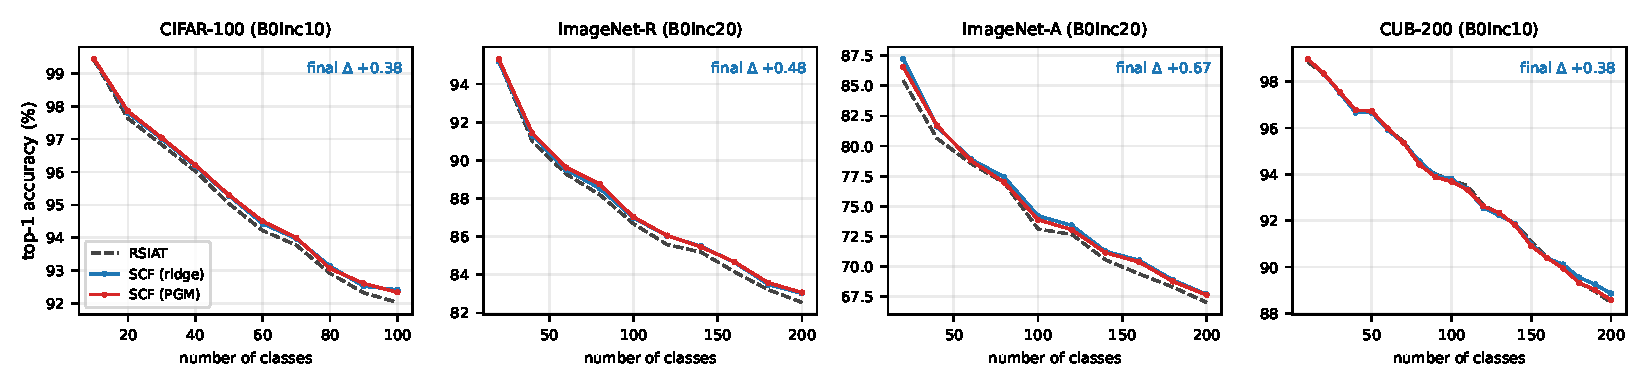
\includegraphics[width=\linewidth]{figures/accuracy_curves.pdf}
\caption{Accuracy after each task as classes accumulate, mean over three
seeds. Dashed: RSIAT. Solid: SCF. The number in each panel is the final gain
of SCF-ridge.}
\label{fig:curves}
\end{figure}

\begin{figure}[t]
\centering
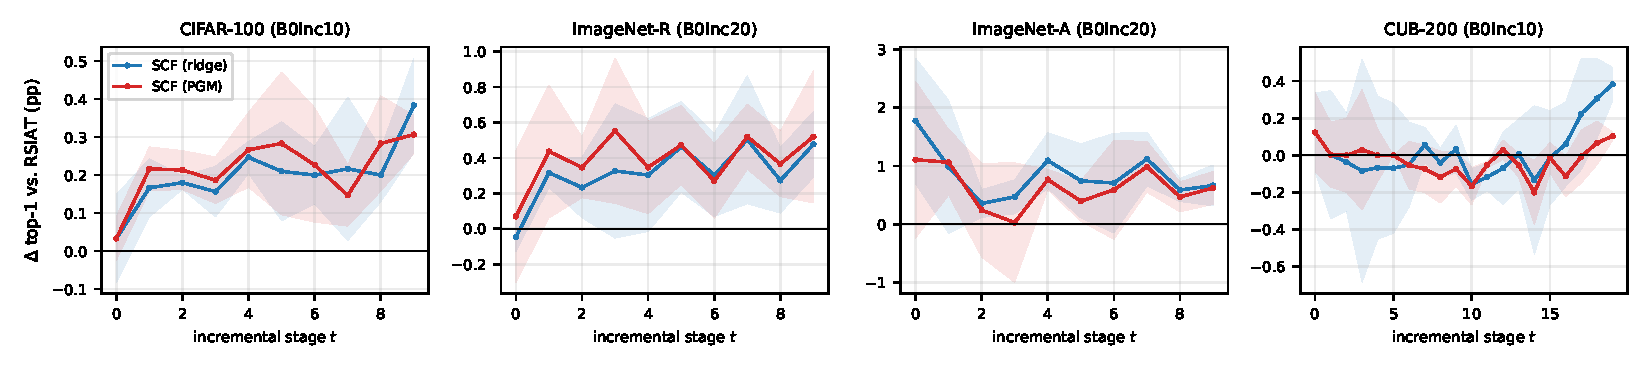
\includegraphics[width=\linewidth]{figures/delta_per_stage.pdf}
\caption{Paired difference to RSIAT at each stage, mean $\pm$ SD over three
seeds. On CIFAR-100, ImageNet-R and ImageNet-A the gain appears at the first
incremental stage and persists. On CUB-200 (20 stages) it appears only in the
last three stages.}
\label{fig:stage}
\end{figure}

\subsection{Analysis}
\label{sec:analysis}

\paragraph{Why CUB-200 gains no average accuracy.}
On CUB-200 the gain is near zero for the first 17 stages. It reaches $+0.22$,
$+0.31$ and $+0.38$ only in the last three (Figure~\ref{fig:stage}). Averaged
over 20 stages, this gives $\bar A\approx0$ while $A_B$ improves. The weight
is not to blame: across the whole grid $w\in\{0.25,\dots,4\}$, no weight gives
CUB-200 a gain above $+0.02$. On this dataset the stored statistics add little
to the CA head until many classes have accumulated. CUB-200 and ImageNet-A
both have about 30 images per class, yet they behave very differently, so
the number of images per class does not predict the gain.

\paragraph{The two heads make different errors.}
Every generative head alone is worse than RSIAT. In $\bar A$ over the three
seeds, ridge alone loses $0.20$ (CIFAR-100), $1.55$ (ImageNet-R), $1.08$
(ImageNet-A) and $0.69$ (CUB-200) points. Still, on ImageNet-R the PGM and
the linear head disagree on $14\%$ of the test images in the final stage:
\begin{itemize}
  \item the linear head is right on $5.8\%$ of the images,
  \item the PGM is right on $3.2\%$,
  \item neither is right on $5.4\%$.
\end{itemize}
Almost all corrections made by the fusion are cross-task errors of the
linear head, the error type identified in Section~\ref{sec:gap}.

\paragraph{The calibration matters.}
Without the scale $\kappa$, adding the CA log-softmax and the PGM
log-probabilities follows the linear head on $87\%$ of the disagreements. The
reason is that Born probabilities are much flatter than a softmax with scale
$s$. That uncalibrated version gained only $+0.25$ (ImageNet-R) and $+0.44$
(ImageNet-A).

\paragraph{Forgetting.}
\begin{table}[t]
\centering
\caption{Forgetting (\%, lower is better), mean over three seeds.}
\label{tab:forgetting}
\setlength{\tabcolsep}{5pt}
\scriptsize
\begin{tabular}{lcccc}
\toprule
Method & CIFAR & IN-R & IN-A & CUB \\
\midrule
RSIAT (ours) & 3.39 & \textbf{5.74} & \textbf{10.44} & 6.77 \\
SCF, ridge & \textbf{3.26} & 5.97 & 11.46 & \textbf{6.20} \\
SCF, PGM & 3.40 & 5.79 & 10.94 & 6.60 \\
\bottomrule
\end{tabular}
\end{table}
Table~\ref{tab:forgetting} reports forgetting. It decreases on CUB-200
($-0.57$, $[-0.79,-0.35]$, ridge), is unchanged on CIFAR-100 and
ImageNet-R, and increases on ImageNet-A ($+1.03$). Forgetting is measured
against each head's own peak accuracy. On ImageNet-A, the fusion raises
the accuracy of a class most at the stage where it is new: averaged over
stages, $+1.60$ on new classes against $+0.53$ on old ones. The peak therefore rises more than the
final value, even though every task ends above RSIAT. We report $\bar A$ and
$A_B$ as the primary measures.

\paragraph{Better statistics are not the lever.}
\begin{itemize}
  \item On ImageNet-R/A, building the PGM states from SSCA-updated means
    instead of the means at learning time helps by only $+0.13$.
  \item Oracle states, recomputed from the old images, lift task~0 by
    $2.8$--$6.5$ points but improve $A_B$ by only $+0.64$.
\end{itemize}
This agrees with Section~\ref{sec:gap}: the representation, not the
statistics, limits what an inference-time rule can recover.
